\documentclass[final,a4paper,10pt]{article}
\usepackage[utf8]{inputenc}
\usepackage[danish]{babel}
\usepackage{natbib}
\bibliographystyle{dk-plainnat}



\usepackage{url}

\usepackage{verbatim}
\usepackage{amsmath}
\usepackage{lscape}
\usepackage{multicol}
\usepackage[draft]{fixme}
\usepackage{tikz}
\usepackage{pgflibrarytikztrees}
\usepackage{lastpage}
\usepackage{listings}
\usepackage{fancyvrb}

\usepackage{wrapfig}                           %Mulighed for at wrappe tekst om figurer
\usepackage{fancyhdr}                          %Flere muligheder med headere og footere
\usepackage{lastpage}                          %Mulighed for at referere til sidste sidetal




\headheight 14.5pt                             %H<F8>jden af headeren
\textwidth 5.87in                              %Tekstbredden

\pagestyle{fancy}                              %Benyt fancyhdr-pakken
\fancyhead[R]{\thepage\ af \pageref{LastPage}} %Skriv sidetallene som "x af y"
\fancyhead[L]{N-dronning problemet i MiG}              %Headeren
\fancyfoot[C]{}                                %Fjern sidetallet som er standard

\oddsidemargin 0.2in                           %Venstre margin er 1in + dette tal
                                               %Med en textwidth p<E5> 5.87in og en
                                               %oddsidemargin p<E5> 0.2 bliver marginerne
                                               %lige store p<E5> A4 som er 8,27in bredt
\font\chessfont=skak10
\def\chs#1{{\chessfont#1}}
\newcommand{\mig}{MiG}
\newcommand{\oc}{One-Click}

\title{Bachelorprojekt\\N-dronning problemet i MiG}
\author{Thomas Clement Mogensen \\ Frej Soya \\ Alex Esmann }

\begin{document}

\maketitle
\tableofcontents

\newpage
\setcounter{page}{1}
\section{Problemformulering}\label{problemformulering}
\begin{verse}
	En del af indholdet af problemformulereringen fra synopsen flyttes til henholdsvis resumé, \ref{nqueenproblemet} og \ref{migogoneclick}. Selve synopsen inkluderes som bilag. Resuméet skal være ren gentagelse.
\end{verse}
%\subsection*{Problemformulering}
Opgavens formål er at implementere en parallel udgave af Takakens algoritme til løsning af n-dronning-problemet. Algoritmen skal køre på MiG-systemet (Minimum Intrusion Grid) og MiG's one-click arkitektur skal kunne udnyttes til at skaffe ressourcer til beregning af problemet. Formålet er på langt sigt at få beregnet en løsning til N-dronning-problemet for $n=26$, men opgaven er kun at gøre dette muligt ved hjælp af MiG. N-dronning-problemet er et klassisk beregningsproblem, der går ud på at finde antallet af mulige måder n dronninger kan placeres på et "skakbræt" med n x n felter, uden at nogen af dem er istand til at slå hinanden i næste træk. Problemets størrelse stiger eksponentielt med n, og er uhyre beregningstungt for store n, hvorfor store distribuerede systemer ofte benyttes. Hidtil er der kun fundet løsninger for $n \in \{1,...,25\}$. For distlab-gruppen her på diku ville en løsning for $n=26$, beregnet på et MiG-grid, kunne skabe opmærksomhed omkring MiG-systemet. 

MiG er beskrevet indgående i \cite{simplemig} og \cite{mig}, \cite{etsi} beskriver N-dronning-problemet grundigere end ovenstående og præsenterer en løsning for n=25. Appendix queens.c i \cite{etsi} er en udskrift af Takakens algoritme implementeret i C.
One-click muliggør deltagelse i et MiG-grid uden andre forudsætninger end en webbrowser og java. Tilgengæld er denne metode begrænset til at afvikle programmer, der er tilgængelige som java-bytecode. Brug af one-click giver adgang til et enormt (potentielt) antal beregningsressourcer, hvilket er grunden til at benytte one-click i denne opgave.    

Opgaven indeholder altså følgende delproblemer: 
\begin{itemize}
\item At finde en effektiv strategi til parallelisering af Takakens algoritme. Herunder overvejelser omkring den optimale størrelse på delproblemer.
\item Implementation af algoritmen i java på en sådan måde at den kan afvikles af one-click-klienter. 
\item Strategi for indsamling, behandling og præsentation af delresultater. 
\item Første opgave er naturligvis at få et bedre kendskab til MiG.
\end{itemize}


\fixme{flyt til oneclick}
One-click muliggør deltagelse i et MiG-grid uden andre forudsætninger end en webbrowser og java. Tilgengæld er denne metode begrænset til at afvikle programmer, der er tilgængelige som java-bytecode. Brug af one-click giver adgang til et enormt (potentielt) antal beregningsressourcer, hvilket er grunden til at benytte one-click i denne opgave.

\fixme{slet?}
 Opgaven indeholder altså følgende delproblemer:
\begin{itemize}
\item At finde en effektiv strategi til parallelisering af Takakens algoritme. Herunder overvejelser omkring den optimale størrelse på delproblemer.
\item Implementation af algoritmen i java på en sådan måde at den kan afvikles af one-click-klienter.
\item Strategi for indsamling, behandling og præsentation af delresultater.
\item Første opgave er naturligvis at få et bedre kendskab til MiG.
\end{itemize}

\subsection{Afgrænsninger}\label{afgraensninger}
%\input{afgraæensninger.tex}

Projektets formål er ikke at beregne en løsning til N-dronning-problemet for $n=26$, hvilket problemets beregningsmæssige omfang kombineret med tids- og ressourcebegræsninger udelukker i praksis. Men kun at muliggøre og forhåbentlig igangsætte denne beregning.
Vi vil ikke tage stilling til den benyttede algoritmes korrekthed eller effektivitet, men kun til den bedst mulige strategi for parallelisering. Partitionering af problemdata skal foregå på en fornuftig måde, med tanke på hvordan det forventes beregningsressourcerne opfører sig, men en decideret statisk undersøgelse af midlertidige MiG-ressourcers opførsel eller levetid vil ikke blive foretaget\footnote{Med ressourcers opførsel tænkes på den tid man kan forvente en bruger vil lade sin one-click-klient køre}. Fordele og ulemper ved MiG eller One-click i forhold til andre grid-systemer falder også udenfor opgavens omfang.

Ved at at løse problemet for et lavere $n$ vil vi kunne estimere tiden og/eller antal CPU'er der skal bruges for at løse for n=26.

\section{Konklusion}\label{konklusion}
\begin{verse}
	Kortfattet konklusion på løsningen og processen
\end{verse}

\section{Nqueen-problemet}\label{nqueenproblemet}

NQueen problemet er finde antallet af måder man kan placere N dronninger på et et kvadratisk NxN bræt, således at ingen dronning kan slå en anden. Bemærk at vi skal finde alle løsninger $Q(n)$, og ikke bare finde alle løsninger - hvilket er et helt andet problem. Hidtil er der kun fundet løsninger for $n \in \{1,...,25\}$.\cite{sekvenser}. Derudover beskriver \cite{etsi} en manuelt distribueret løsning for $n=25$. Der findes desuden masser af referencer på \url{http://www.liacs.nl/home/kosters/nqueens.html} relateret til nqueen problemet. 


\begin{figure}
\begin{center}
\begin{tabular}{|c|c|c|c|c|c}
\hline	 &  & &   \chs{q} & \\
\hline	\chs{q} & &  &  & \\
\hline	 & & \chs{q} &  &  \\
\hline	 &  &  & & \chs{q} \\
\hline	 & \chs{q} & &  &  \\
\hline
\end{tabular}
\end{center}
\caption{Eksempel på en løsning for $n=5$}
\end{figure}


\subsection{Backtracking}\label{backtracking}

En 

\fixme{Træstruktur kunne være endnu bedre med et grid i hver knude der viser valgte pladser med en markering}

\begin{tikzpicture}[node distance=1cm]
	%    \tikzstyle{every node}=[draw]    
	\node (root) {} child {edge from parent};
\end{tikzpicture}


\begin{figure}[!h]

\begin{tikzpicture}[node distance=1cm]
	%    \tikzstyle{every node}=[draw]
    \node (root) {} [grow=right]
   	    child 
   	    child 
	    child
    	child {node (2) {2}
	        child  {node (25) {5}
    	  		child {node  {3}
    	  			child { node{1} child { node{4}} }
	      		}
    	   		child {node {1} child {node{4}}}        		        	          		        	  
	       	}
		    child {node {4}
		    	child {node {1}
		    		child {node {3} child { node {5}} }
		    	} 
		    }
	     }
	     child 
	 ;

\end{tikzpicture}
\caption{Ovenstående løsning hvor vi allerede har valgt 2 i række 1, kan den følgende udregning vises som et træ.
Antallet af børn er antallet af \textit{mulige} valg som ikke blokeres af tidligere placeringer}
	
\end{figure}



\subsection{Bitmapmodellen}\label{bitmapmodellen}
\begin{verse}
	Beskrivelse af NQueen problemet som bitmaps / bit vektorer
\end{verse}

Samme bræt repræsenteres som et binært mønster. \textbf{1} markerer placering af en dronning. Det totale antal løsninger er begrænset af $n!$. 
Et bræt med en eller flere valgte linjer kan løses på samme måde med takakens algoritme. Hvert delbræt kan løses uafhængigt og antallet af løsninger for hvert bræt akkumuleres for at få det totale antal løsninger.

Dette kan gentages for hver linje. Ved at oprette delbræt hvor M linjer allerede er valgt. Findes ca. (N-M)! delbræt skal der for N=26 vil der for M=3 være 26*25*24=15,600 delbræt.

Dette er en øvre grænse, der oprettes ikke delbræt som ikke er gyldige, og derudover er der i takakens kode optimeringer så der kun findes unikke løsninger (som så kan roteres og eller spejles)


\subsection{Takakens backtrack optimeringer}\label{backtrackoptimeringer}
\begin{verse}
	Vi har afgrænset os fra at beskrive Takakens optimeringer, endsige vise deres korrekthed. I dette afsnit vil vi dog alligevel diskutere optimeringernes overordnede virkemåde. Dog kun i det omfang det er nødvendigt for at kunne omstrukturere algoritmen uden at miste optimeringer.   
\end{verse}

Takaken opdeler beregningen i to delproblemer. Et hvor den første dronning placeres i øverste hjørne, og et andet delproblem hvor dronningen placeres i midten. For løsninger med dronninger i hjørnet fjernes løsninger i kolonne 2 fra fra$2 \ldots n-2$. 


\subsection{Sikkerhed}

\section{MiG og one-click}\label{migogoneclick}
\begin{verse}
	Her beskrives MiG-grid og one-click overordnet. Tekniske detaljer i forbindelse med brug af MiG-grid, og særligt udvikling af one-click-applikationer, identificeres. Dette afsnit henvender sig således kun til dig, der ikke allerede har kendskab til disse emner.  
\end{verse}

\subsection{Minimum intrusion Grid}\label{mig}

Minimum instrusion Grid, herefter MiG, er et grid-system der sigter efter at stille så få krav til deltagelse som muligt - både for brugere og ressourcer. I MiG-termiologi en ressource en enhed der kan sættes til at beregne et problem. I mange andre gridsystemer benyttes speciel software til kommunikation mellem den enkelte ressource og gridet, undgår man helt dette mindskes kompleksiteten af det samlede system dramatisk. Omkostninger til den første opsætning og efterfølgende vedligeholdelse af systemet minimeres.   \fixme{beskrivelse af anonymitet, sikkerhed, skalerbarhed, 	referér til artikler på migrid.org}. MiG er beskrevet indgåede på i \cite{simplemig,mig}

MiG giver brugeren mulighed for at få adgang til et stort antal beregningsressourcer, uden at skulle bekymre sig om hvor disse befinder sig, hvem der ejer dem, hvorvidt de hver især er istand til at løse den aktuelle opgave\footnote{Et givent problem kan f.eks. stille særlige krav til ressourcens arkitektur, eksisterende programmel, osv. }\fixme{footnote er der mere under osv?}. Her og i det nedenstående skal "brugeren" læses som "en person/udvikler m/k der ønsker at få beregnet et problem vha. MiG \fixme{mindre fjollet definition}. Brugeren præsenteres for en abstraktion af MiG, der fremstiller et kendt paradigme fra unix-systemer; et hjemmekatalog hvori brugeren kan placere sine data- og programfiler. Brugerens interaktion med MiG forgår via en række scripts der efterligner kendte kommandoer til manipulation af filer i hjemmekataloget, og introducerer kommandoer til at starte og stoppe job. Begge metoder giver mulighed for at udføre basale funktioner på MiG, såsom at igangsætte job, se status på tidligere jobs og give adgang til data-, program- og resultatfiler i hjemmekataloget. Et job sættes igang ved at køre kommandoen migsubmit med såkaldt mRSL-fil\footnote{MiG Resource Selector Language} der indeholder en beskrivelse af det job der skal afvikles. Beskrivelsen fortæller MiG hvilken programfil der skal køres, med hvilke parametre, hvor lang tid jobbet forventes at tage og eventuelle krav jobbet har til ressourcer der skal afvikle det. Et kørende job har adgang filerne i  hjemmekataloget. Resultatet af et job skal skrives til hjemmekataloget for senere at kunne aflæses af brugeren. For hvert job oprettes desuden 3 filer i hjemmekataloget. De indeholder hhv. exit-status, standard output og standard error, ganske som de kendes fra unix-systemer. 
Al den ovennævnte interaktion med MiG kan alternativt foregå gennem et særligt webinterface. 
Vores system har flere dele, selve Grid delen er MiG som for os er en lukket boks
Da en delopgave specifikt er at bruge og afprøve OneClick som kører som en java Applet.

TODO: Andre system ting?

\subsection{OneClick Applet}\label{applet}

OneClick er et framework til udvikling af java-appletter, der kan interagere med MiG. Ved hjælp af OneClick kan en hvilken som helst computer gøres til en MiG-ressource, unden nogen for for opsætning eller installation af programmel, hvilket gør det muligt for ganske alm. mennesker at bidrage regnekraft til gridet. Det eneste der kræves er en webbrowser der kan afvikle java-appletter. Implementerer man sit job som en java-applet vil det kunne afvikles på alle OneClick-ressourcer, uden at skulle specificere særlige krav til arkitektur med videre. Til gengæld vil det være begrænset til kun at køre på OneClick-ressourcer. 
OneClick er især interessant i forbindelse med hvad man kunne kalde sociale beregninger, det vil sige beregningsprojekter som almindelige mennesker kunne have interesse i at bidrage til, eller endog konkurrere om at bidrage mest til. Kendte eksempler på sådanne projekter er SETI@home og FOLDING@home. Når måling af tidsforbrug per resource bliver implementeret i OneClick kunne man også  forestille sig et MiG-grid som en åben markedsplads hvor både virksomheder og privatpersoner kunne købe og sælge regnekraft gennem MiG uden at skulle bekymre sig om hvor beregningerne reelt foretages eller hvad hvad der regnes på.  \fixme{blah-blah}

Ved afvikling af java-appletter er der en række begrænsinger pga, applets
\begin{itemize}
	
	\item Sandbox model
	\item max 64 mb ram
	\item OneClick Kode/Mininum intrusion
\end{itemize}

\section{Paralellisering af Takaken's nqueen I Java}

\subsection{Generelle implementeringsovervejelser}
\subsubsection{Opdeling af opgaver}

\begin{itemize}
\item{Vi er nødt til at tage højde for at løsningen (antallet af løsinger) vil overstige hvad vi kan repræsentere som en 32bit værdi. }
\end{itemize}

I forbindelse med joboprettelse og resultatindsamling skal vi træffe nogle valg mht.
\begin{itemize}
\item{Joboprettelsesstrategi - hvad skal der til for at beskrive et job.}
\item{}
\end{itemize}

\subsection{One-click-specifikke begrænsninger}

Class-filer caches af browserens java-plugin. Ændringer i class-filer, der betyder opdatering af serialVersionUID, kræver at browseren genstartes for ikke at fejle på serialVersionUID og derved færdiggøre jobbet, men uden resultat! 

\subsubsection{Bugs og mangler}
\begin{itemize}
	\item Et job fejler ikke hvis jobbet kaster en java.lang.Error (Forskellig fra Java.lang.Exception, begge har dog typen java.lang.Throwable)
	\item Ens job tvinges til at afhænge af MiG.nqueen.JoB
	\item File I/O følger ikke Inputstream / Outputstream	
	\item Brug af suns egen HTTP implementation. Brug i stedet http-commons fra Apache
	\item Vi har glemt en masse
	\item Webstart vil klart være at foretrække. Det er rigtigt at der kommer en certifikat fejl (https) - men så længe certifikat ikke er i browserens CA liste vil browseren i stedet komme med en advarsel.
\end{itemize}


\subsection{Konkrete implementeringsproblemer}
\subsubsection{Mig job}\label{label}
\subsubsection{Iterative udgave}
\subsection{Checkpoint}

Fordi checkpointing gemmer ikke stack.


\subsection{Resultatindsamling og -visning}
Vi skal have en vedligeholdelsesproces kørende, der sørger for at 

- Frej Lad mig sende en mail pr. færdigt job? Og så et job der checker 'jævnligt' at alle mails er modtaget?


\subsection{Resultatindsamling og -visning}
En måde et holde styr på den samlede beregning af en løsning på n-dronning-problemet er, at have en vedligeholdelsesproces kørende, der sørger for at 
\begin{itemize}
	\item Genkøre fejlede job
	\item Indsamle resultater fra færdige jobs
	\item Muliggøre løbende projektstatus og offentliggørelse af resultater 
\end{itemize}
Dette program kan for eksempel være det samme der står for at oprette vores jobs i første omgang. Muligheden for at tilpasse ikke-kørte jobs på baggrund af informationer om gridets tilstand (antallet af tilgængelige resourcer). 

Som alternativ tilbyder migrid at informere indsendere når dennes job er afsluttet, eksempelvis via email. Det vil være betydeligt enklere kun at foretage behandling af resultater hver gang et sådant er klar, uden at have et permanent indsamlingsprogram kører. Vi er dog stadig nødsaget til at håndtere fejl i det enkelte job eller rapporteringen af jobafslutning. 



\section{Implementeringens struktur}\label{implementeringensstruktur}
\begin{verse}
	Følgende er ment som en læsevejledning til programmets kildekode, såvel som en vejledning til afvikling af programmet til forskellige formål. 
\end{verse}

Den udviklede kildekode er organiseret i følgende filer:
\begin{itemize}
	\item[Board.java] 
	\item[Board2.java] Basis-klasse for wrapper-klasser til backtrack
	\item[CornerBoard.java] wrapper-klasse til backtrack for cornerboards
	\item[MiddleBoard.java] wrapper-klasse til backtrack for middleboard
	\item[CheckPointer.java] implementerer checkpointing
	\item[CheckPointAction.java] implementerer checkpointing
	\item[CornerBoardTest.java] unittests til CornerBoard
	\item[MiddelBoardTest.java] unittests til MiddleBoard
	\item[MiGClient.java] java-implementation af en del af migrid-hjælpeprogrammerne
	\item[MiGJob.java] klasse der beskriver et job og kan generere en .mRSL-fil
	\item[MiGSSLSocketFactory.java] hjælpeklasse til MiGClient-klassen
	\item[NQueenBoards.java] Jobgeneratoren, parallel-nqueen-algoritme, der genererer delproblemer i form af boards, hvor de første $m$ dronninger allerede er placeret. 
	\item[NQueenJob.java] hovedklassen for et migrid-one-click-job. 
	\item[NQueens.java] Testfil - Direkte java-port af Takakens c-kode. Kan køres som one-click job.
	\item[NQueensL.java] Testfil - Direkte java-port af Takakens c-kode. Kan køres lokalt.
\end{itemize}

Programmet kan afvikles lokalt på en enkelt maskine eller på migrid,  



\section{Afprøvning og benchmarking}
%Benchmarking-delens fremmeste formål er at finde svar på en række spørgsmål inden udregningen sættes igang.
%Reelt har vi kun en enkelt parameter vi kan skrue på, nemlig $m$ - antallet af dronninger vi placerer på hver board før vi genererer et mig job til at regne videre på det board. 
%Hvilket forhold mellem 

%\subsection{Takaken}
%\subsection{Java port}
%\subsection{Java port v2}
%\subsubsection{Rekursion vs. Iterativ metode}
%\subsubsection{Iterativ med checkpoints}
%\subsection{MiGrid}

Benchmarking-delens fremmeste formål er at finde svar på en række spørgsmål
inden udregningen sættes igang.  Reelt har vi kun en enkelt parameter vi kan
skrue på, nemlig $m$ - antallet af dronninger vi placerer på hver board før vi
genererer et mig job til at regne videre på det board.  Hvilket forhold mellem 
\fixme{what?}
%\subsection{Takaken}
%\subsection{Java port}
%\subsection{Java port v2}
%\subsubsection{Rekursion vs. Iterativ metode}
%\subsubsection{Iterativ med checkpoints}
%\subsection{MiGrid}

\subsection{Lokale tests}

Vi starter med at teste de forskellige udgaver af koden lokalt, så vi har en
baseline at sammenligne med.

Alle lokale tests er kørt på en IBM T43, med en pentium m 1.86Ghz cpu, 

Java koden er kompilet med javac

\begin{verbatim}
alex@roadrunner:~/temp/queens/src/main/java$ javac -version
javac 1.5.0_11
\end{verbatim}

C koden er kompilet med \texttt{gcc -Os -O2 -o nq nqueens.c}

\begin{verbatim}
alex@roadrunner:~/temp/queens/src/main/java$ gcc --version
gcc (GCC) 4.1.2 (Ubuntu 4.1.2-0ubuntu4)
\end{verbatim}

De første tests er kørt på revision 77 (i forbindelse med den iterative test er
udskrivning af debug info til skærmen dog blevet kommenteret ud)

\begin{figure}[h]
\begin{center}
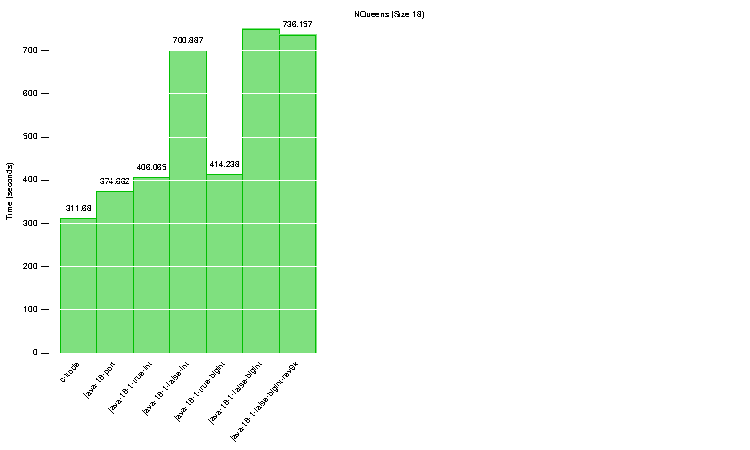
\includegraphics{../benchmarks/lokal.pdf}
\caption{insert proper caption here } 
\label{figur:lokal}
\end{center}
\end{figure}
\fixme{caption, or no caption.. this graph is redundant information}

Som det ses er C udgaven en smule hurtigere end den direkte java port, der igen
er lidt hurtigere end den paralleliserede udgave af koden, når den kører
rekursivt. Den iterative udgave er væsentlig langsommere..

Den parallelle udgave af koden er i dette tilfælde her kørt med
\texttt{maxSteps} på 1. 
\begin{figure}[h]
\begin{center}
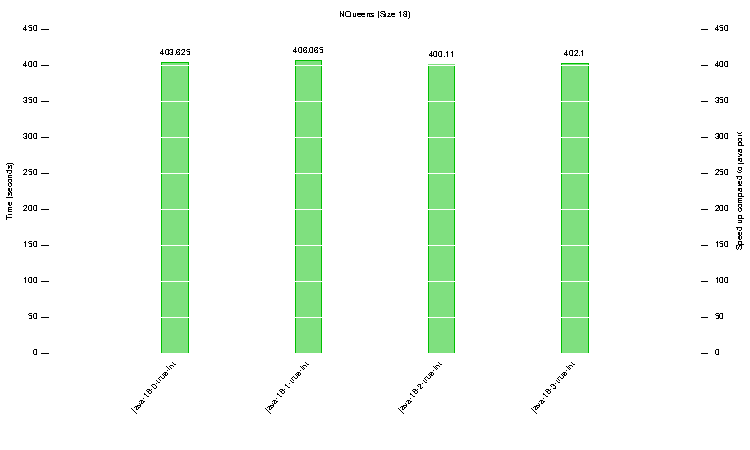
\includegraphics{../benchmarks/maxsteps.pdf}
\caption{insert proper caption here } 
\label{figur:maxsteps}
\end{center}
\end{figure}

På figur \ref{figur:maxsteps} er vidst kørsler for $n=18$ for forskellige
$maxSteps$. 
Som det ses, har det ikke den store indflydelse på performance hvor stor
$maxSteps$ er, der er altså ikke det store overhead ved at generere en masse
opgaver og løse dem bagefter, når det kører lokalt. 

Det skal også nævnes at for $maxSteps>n/2$ vil vores program regne forkert.
Dette skyldes \fixme{ja.. hvad skyldes det.. }


I tabel \ref{tabel:noboards} kan det ses hvor mange boards der bliver genereret
for forskellige $n$ og $maxSteps$. 

\fixme{hvor mange jobs bliver der lavet for de forskellige maxsteps, indsæt
tabel?}
\begin{table}
	\begin{center}
		\begin{tabular}{|c|c|c|c|c|c|}
			\hline N  & maxSteps  & boards & n  & maxSteps & boards \\
			\hline 15 & 0         & 18     & 17 & 0        & 21     \\
			\hline 15 & 1         & 173    & 17 & 1        & 243    \\
			\hline 15 & 2         & 1310   & 17 & 2        & 2282   \\ 
			\hline 15 & 3         & 8349   & 17 & 3        & 18161  \\
			\hline 15 & 4         & 43961  & 18 & 0        & 23     \\
			\hline 16 & 0         & 20     & 18 & 1        & 289    \\
			\hline 16 & 1         & 212    & 18 & 2        & 2983   \\
			\hline 16 & 2         & 1797   & 18 & 3        & 26204  \\
			\hline 16 & 3         & 12840  &    &          &        \\
			\hline 16 & 4         & 76224  &    &          &        \\
			\hline
		\end{tabular}
		\caption{Antal Boards der bliver genereret}
		\label{tabel:noboards}
	\end{center}
\end{table}

Alle tests er i første omgang kørt 5 gange, dette blev gjort for at se om
køretiden svingede meget, da dette ikke lader til at være tilfældet (se figur
\ref{figur:b1} vil resten af testene kun blive kørt 1 gang.. 

\begin{figure}[h]
\begin{center}
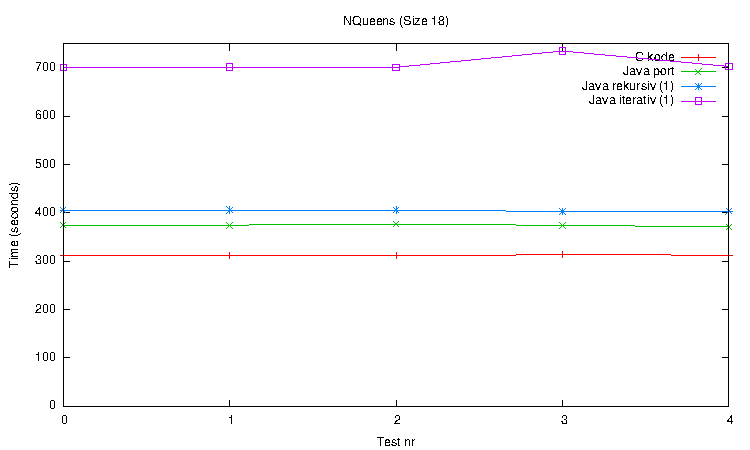
\includegraphics{../benchmarks/b1.pdf}
\caption{insert proper caption here } 
\label{figur:b1}
\end{center}
\end{figure}

Nu skal vi så se på hvor hurtigt det kører når vi smider det efter MiGrid. 
Disse tests er kørt med \texttt{maxSteps} 0 og 1.

\fixme{indsaet en graf, eller bare resultaterne og henvis til b3?}
De foregående tests er kørt med kode der bruger \texttt{int} til at gemme resultaterne,
i de næste tests er \texttt{int} skiftet ud med \texttt{BigInteger} (revision
83
\clearpage
Sammenligning af alle benchmarks

Som det ses på figur \ref{figur:lokal} kører den iterative udgave af koden fra
rev. 83 (med bigint) utroligt langsomt i forhold til foregående udgaver.  Dette
skyldes en en linje kode, der ikke var blevet kommenteret ud. Denne linje
konkatenerede to strenge. Uden denne linje kører koden væsentlig hurtigere, som
det kan ses på den sidste søjle i figur \ref{figur:lokal}


Som det kan ses på figur \ref{figur:lokal} kører den rekursive kode en smule
langsommere med \texttt{BigInteger} end med \texttt{int}, hvor tiden stiger fra
406.xxx til 414.xxx\fixme{indsaet rigtige tal}, hvilket svarer til en forøgelse
på knap 2\%

\subsection{overhead ved jobskifte}

I MiG\_main() metoden i NQueenJob laver vi et timestamp i starten og slutningen
af metoden.  og kan så tage start tiden for et job og trække sluttiden for det
foregående job fra, og man har så et estimat for hvor lang tid et jobskifte
tager, vi har gjort dette for 8 jobs, og får så 7 estimater, gennemsnittet af
dem bliver 18.455 sek.  Op til 15 af disse 18 sekunder, skyldes at oneclick
applet'en sover i 15 sekunder.  Ved en kørsel med $n=18$ og $maxSteps=1$, hvor
vi så får 289 jobs, giver det knap 89 minutter. 

\subsection{kald til backtrack}

Hvis man ser på antallet af kald til backtrack de forskellige versioner laver,
er de ens for c koden og den direkte java port, og hvis man kører med
$maxSteps=0$ er antallet af kald for den parallele og iterative kode også det
samme som for c koden (se tabel \ref{tabel:backtrackkald}. Med $maxSteps>0$ får
vi færre kald til backtrack, hvilket skyldes at en del af disse kald bliver
lavet i forbindelse med oprettelsen af de ekstra boards. 

\begin{table}
\begin{center}
\begin{tabular}{|c|c|c|c|}
\hline 18 & C kode        &             &             \\
\hline 18 & Java          &             &             \\
\hline 18 & Java rek. &             &             \\
\hline 18 & Java ite. &             &             \\
\hline
\end{tabular}
\caption{Kald til backtrack}
\label{table:backtrackkald}
\end{center}
\end{table}
\fixme{indsæt tal (*07-01*)}

\subsection{Jobstørrelse}

Med jobstørrelse refererer vi til hvor lang tid det tager at løse et job, og
ikke størrelsen på data. 
Som det ses i \ref{tabel:jobsize}, varierer jobstørrelsen
meget. Cornerboards er generelt ret små, mens middleboards er generelt er en del
større. Det ses også i tabellen at jobstørrelsen afhænger af de bounds der er i
henholdsvist MiddleBoard og CornerBoard. Hvis man øger $maxSteps$ og dermed får
lavet flere jobs, ses det at de enkelte jobs bliver delt op i nogenlunde lige
støre dele, den relative størrelse mellem det mindste og største jobs er dog
stadig nogenlunde det samme. \fixme{lav en benchmark/beregning der viser dette?}

\subsection{Generering af jobs}

Generering og indsendelse af jobs afhænger tildels af den internetforbindelse
man sidder på, da indsendelse jo går via internettet. De forskellige jobs vi har
submitted til MiGrid har genereringen og indsendelse af jobs svinget fra xx til
xx (se tabel \ref{tabel:jobgenerering}) \fixme{lav den fscking tabel og skriv de
rigtige tal ind}. Langt den største del af tiden går også med at sende jobsne,
da genereringen af jobs for større mængder jobs tager ca 0.01ms/job
\begin{verbatim}
18: 4, 6, 44, 280
18: 23, 289, 2983, 26204
18: 0.17, 0.02, 0.01, 0.01
17: 4, 6, 23, 206, 1252
17: 21, 243, 2282, 18161, 121116
17: 0.19, 0.02, 0.01, 0.01, 0.01
\end{verbatim}
\fixme{lav det om til en tabel.. der}

TODO
\section{Forbedringer til OneClick}
%\input{forbedringer.tex}
TODO


%\bibliographystyle{plainnat}


\bibliography{rapport}

\appendix
%\landscape
%\tiny


\section{Kildekode}
\subsection{nqueens.c}
%\verbatiminput{../../nqueens.c}

\section{Synopsis}
%\documentclass[a4wide,10pt]{article}

\usepackage[danish]{babel}
\usepackage[latin1]{inputenc}
\usepackage{verbatim}
\usepackage{amsmath}
\usepackage{lscape}
\usepackage{multicol}

\title{Bachelorprojekt\\Synopsis\\N-dronning problemet i MiG}
\author{Thomas Clement Mogensen \\ Frej Soya \\ Alex Esmann }

%\maketitle
\begin{document}
\maketitle

\subsection*{Problemformulering}
Opgavens formål er at implementere en parallel udgave af Takakens algoritme til løsning af n-dronning-problemet. Algoritmen skal køre på MiG-systemet (Minimum Intrusion Grid) og MiG's one-click arkitektur skal kunne udnyttes til at skaffe ressourcer til beregning af problemet. Formålet er på langt sigt at få beregnet en løsning til N-dronning-problemet for $n=26$, men opgaven er kun at gøre dette muligt ved hjælp af MiG. N-dronning-problemet er et klassisk beregningsproblem, der går ud på at finde antallet af mulige måder n dronninger kan placeres på et "skakbræt" med n x n felter, uden at nogen af dem er istand til at slå hinanden i næste træk. Problemets størrelse stiger eksponentielt med n, og er uhyre beregningstungt for store n, hvorfor store distribuerede systemer ofte benyttes. Hidtil er der kun fundet løsninger for $n \in \{1,...,25\}$. For distlab-gruppen her på diku ville en løsning for $n=26$, beregnet på et MiG-grid, kunne skabe opmærksomhed omkring MiG-systemet. 

MiG er beskrevet indgående i \cite{simplemig} og \cite{mig}, \cite{etsi} beskriver N-dronning-problemet grundigere end ovenstående og præsenterer en løsning for n=25. Appendix queens.c i \cite{etsi} er en udskrift af Takakens algoritme implementeret i C.
One-click muliggør deltagelse i et MiG-grid uden andre forudsætninger end en webbrowser og java. Tilgengæld er denne metode begrænset til at afvikle programmer, der er tilgængelige som java-bytecode. Brug af one-click giver adgang til et enormt (potentielt) antal beregningsressourcer, hvilket er grunden til at benytte one-click i denne opgave.    

Opgaven indeholder altså følgende delproblemer: 
\begin{itemize}
\item At finde en effektiv strategi til parallelisering af Takakens algoritme. Herunder overvejelser omkring den optimale størrelse på delproblemer.
\item Implementation af algoritmen i java på en sådan måde at den kan afvikles af one-click-klienter. 
\item Strategi for indsamling, behandling og præsentation af delresultater. 
\item Første opgave er naturligvis at få et bedre kendskab til MiG.
\end{itemize}

Projektets form�l er ikke at beregne en l�sning til N-dronning-problemet for $n=26$, hvilket problemets beregningsm�ssige omfang kombineret med tids- og ressourcebegr�sninger udelukker i praksis. Men kun at muligg�re og forh�bentlig igangs�tte denne beregning. 
Vi vil ikke tage stilling til den benyttede algoritmes korrekthed eller effektivitet, men kun til den bedst mulige strategi for parallelisering. Partitionering af problemdata skal foreg� p� en fornuftig m�de, med tanke p� hvordan det forventes beregningsressourcerne opf�rer sig, men en decideret statisk unders�gelse af midlertidige MiG-ressourcers opf�rsel eller levetid vil ikke blive foretaget\footnote{Med ressourcers opf�rsel t�nkes p� den tid man kan forvente en bruger vil lade sin one-click-klient k�re}. Fordele og ulemper ved MiG eller One-click i forhold til andre grid-systemer falder ogs� udenfor opgavens omfang. 


\begin{thebibliography}{99}
\bibitem{simplemig} Karlsen, Henrik Hoey, Vinter, Brian:
\emph{Minimum intrusion Grid - The simple model},
http://mig-1.imada.sdu.dk/MiG/Mig/published\_papers/ETN05-Simple.pdf (2005)
\bibitem{mig} Vinter, Brian:
\emph{The Architecture of the Minimum intrusion Grid, MiG},
http://mig-1.imada.sdu.dk/MiG/Mig/published\_papers/CPA05-Arch.pdf
(2005)
\bibitem{etsi} Guillemin, Patrick:
\emph{3rd N Queens ETSI Plugtests Contest - Counting the number of
  solutions Single and Distributed Programs}
http://portal.etsi.org/docbox/GRID/Open/GRID\%20Plugtests\%202006/N-QUEENS-TESTCASE-2006-v2.pdf (2006)
\end{thebibliography}

%\landscape
%\tiny
%\begin{multicols}{2}[\section{\LaTeX kildekode}]
%\section*{Skabelon.tex}
%\verbatiminput{skabelon.tex}
%\end{multicols}

\end{document}




%\begin{multicols}{2}[\section{\LaTeX kildekode}]
%\section*{Skabelon.tex}
%\verbatiminput{skabelon.tex}
%\end{multicols}


\end{document}
